\documentclass[11pt]{beamer}
\mode<presentation>
\let\Tiny=\tiny
\usetheme{CambridgeUS}
\usefonttheme{professionalfonts}
\usepackage[brazil]{babel}
\usepackage[utf8]{inputenc}
\usepackage{amsfonts}
\usepackage{amssymb}
\usepackage{amsmath}
\newtheorem{mydef}{Definição}
\newtheorem{myexample}{Exemplo}
\usepackage{listings}
\usepackage{fancyvrb}
\usepackage{enumerate}

\lstset{basicstyle=\scriptsize,language=Java, showstringspaces=false}

\newcommand\blfootnote[1]{%
  \begingroup
  \renewcommand\thefootnote{}\footnote{#1}%
  \addtocounter{footnote}{-1}%
  \endgroup
}

\title{Arquitetura do Sistema de Bancos de Dados}
\author{}
\date{}

\begin{document}

\begin{frame}[plain]
    \titlepage
\end{frame}

\section{Arquitetura cliente/servidor}

\begin{frame}{Arquitetura cliente/servidor}
    \begin{itemize}
        \item A arquitetura mais comum em sistemas de bancos de dados é a arquitetura cliente/servidor de 2 ou 3 camadas.
        \item O módulo cliente corresponde às aplicações e usuários que acessam o banco.
        \item O SGBD atua como um servidor de consultas ou transações, sendo responsável pelo armazenamento, acesso e busca dos dados.
    \end{itemize}
\end{frame}

\begin{frame}{Arquitetura cliente/servidor}
    \begin{itemize}
        \item O servidor fornece uma API (\textit{Application Programming Interface}) que permite que os clientes se autentiquem no banco e façam requisições.
        \item O padrão ODBC (\textit{Open Database Conectivity}) define quais serviços serão ofertados e como deve ser feita a conexão entre cliente e servidor.
        \item Deste modo, basta trocar o \textit{driver} do SGBD para trocar de um SGBD para outro.
    \end{itemize}
\end{frame}

\begin{frame}{Arquitetura cliente/servidor}
    \begin{itemize}
        \item Com o crescimento das aplicações \textit{web}, foi inserida uma terceira camada intermediária.
        \item Esta camada é o servidor de aplicação, que recebe a requisição HTTP do cliente e estabelece ele mesmo a conexão com o SGBD (servidor de consultas).
        \item \textit{Frameworks} modernos como Spring Boot (Java), Laravel (PHP), Django (Python) e Rail (Ruby) usam o princípio de \textit{convention over configuration} para tornar mais abstrata ainda a comunicação com o banco de dados.
        \item Estes \textit{frameworks} possuem mapeadores objeto-relacionais que permitem que o desenvolvedor use pouca SQL (\textit{Structured Query Language})\footnote{Linguagem padrão dos bancos de dados relacionais.}.
    \end{itemize}
\end{frame}

\begin{frame}{Arquitetura cliente/servidor}
    \begin{itemize}
        \item Salienta-se que a arquitetura cliente/servidor é a arquitetura vista de alto nível.
        \item Ela define as responsabilidades dos dois ou três agentes (camadas), mas não define como cada um funcionará.
    \end{itemize}
\end{frame}

\section{Modelos de dados}

\begin{frame}{Modelos de dados}
    \begin{itemize}
        \item O banco de dados\footnote{Quando falamos banco de dados nos referimos a estrutura e organização dos dados e seus valores.} pode funcionar com diferentes camadas de abstração.
        \item Cada camada é conhecida como modelo de dados.
    \end{itemize}
\end{frame}

\begin{frame}{Modelos de dados}
    São três os tipos de modelos de dados:
    \begin{itemize}
        \item conceituais;
        \item representativos;
        \item físicos.
    \end{itemize}
\end{frame}

\begin{frame}{Modelos de dados conceituais}
    \begin{itemize}
        \item Os modelos de dados conceituais são os de mais alto nível.
        \item O modelo Entidade-Relacionamento (ER) é o modelo conceitual mais utilizado ainda para definir um banco de dados neste nível.
        \item Entretanto, modelos baseados em classes, utilizando ou não linguagens de modelagem como a UML (\textit{Unified Modeling Language}) possuem bastante espaço devido aos mapeadores objeto-relacionais.
    \end{itemize}
\end{frame}

\begin{frame}{Modelos de dados representativos}
    \begin{itemize}
        \item Os modelos representativos são modelos intermediários, pois oferecem conceitos que estão mais próximos da máquina, porém ainda são bastante inteligíveis aos usuários finais.
        \item O modelo representativo ainda dominante é o modelo relacional.
    \end{itemize}
\end{frame}

\begin{frame}{Modelos de dados físicos}
    \begin{itemize}
        \item Os modelos de dados físicos descrevem como os dados serão armazenados.
        \item Eles também descrevem como serão realizadas as indexações dos dados.
    \end{itemize}
\end{frame}

\begin{frame}{Modelos de dados}
    \begin{itemize}
        \item É importante lembrar que os modelos de dados definem o esquema do banco de dados, ou seja, a organização estrutural dos dados.
        \item Eles não definem o estado do banco, que corresponde ao conjunto de valores do banco de dados.
        \item Os modelos de dados são bastante importantes no projeto de bancos de dados, pois o modelo conceitual permite a discussão em alto nível com os \textit{stakeholders}.
        \item Já o modelo representativo pode ser obtido através da derivação do modelo conceitual e permitem que os programadores implementem o esquema definido.
    \end{itemize}
\end{frame}

\section{Arquitetura de três esquemas}

\begin{frame}{Arquitetura de três esquemas}
    \begin{itemize}
        \item Um comitê denominado ANSI/SPARC definiu um padrão arquitetural que até hoje serve de guia para os fabricantes de SGBDs.
        \item O padrão define 3 níveis:
              \begin{itemize}
                  \item nível externo;
                  \item nível conceitual;
                  \item nível interno.
              \end{itemize}
    \end{itemize}
\end{frame}

\begin{frame}{Arquitetura de três esquemas}
    \begin{itemize}
        \item O nível externo é composto pelas visões do banco de dados que serão ofertadas aos usuários/aplicações.
        \item O nível conceitual é de nível intermediário, pois define o esquema conceitual, ou seja, é uma abstração sobre o nível interno, porém com alguns aspectos vinculados ao mesmo.
        \item O nível interno descreve a estrutura de armazenamento interno do banco de dados.
    \end{itemize}
\end{frame}

\begin{frame}{Arquitetura de três esquemas}
    \begin{itemize}
        \item Apesar de ser padrão, a implementação da arquitetura ANSI/SPARC varia de acordo com o SGBD.
        \item Em alguns SGBDs é possível até mesmo o uso de modelos de dados diferentes para os níveis externo e conceitual.
        \item Pode-se utilizar o modelo orientado a objetos para o nível externo e relacional para o nível conceitual, como faz o UDB da IBM.
    \end{itemize}
\end{frame}

\begin{frame}{Arquitetura de três esquemas}
    \begin{itemize}
        \item A segregação entre as camadas permite a independência lógica e física dos dados.
        \item Entretanto, a necessidade de mapeamento entre os níveis diminui a performance do banco de dados.
    \end{itemize}
\end{frame}

\section{Arquitetura de sistema de bancos de dados}

\begin{frame}{Arquitetura de bancos de dados}
    \begin{itemize}
        \item Apesar de parecidos, os conceitos de arquitetura cliente/servidor, modelos de dados e arquitetura ANSI/SPARC trabalham em níveis de abstração diferentes.
        \item A arquitetura cliente/servidor oferece uma visão macro, pois organiza a aplicação, os usuários e o SGBD, mas sem oferecer detalhes internos.
        \item Já os modelos de dados conceitual e representativo servem para definir especialmente o esquema do banco de dados (nível conceitual da arquitetura ANSI/SPARC).
        \item Eles também podem ser utilizados para definir o nível externo da arquitetura ANSI/SPARC.
        \item O modelo de dados físico e o nível interno da ANSI/SPARC se sobrepõem e geralmente são tratados pelo próprio SGBD.
    \end{itemize}
\end{frame}

\section{Linguagens dos sistemas de bancos de dados}

\begin{frame}{Linguagens dos sistemas de bancos de dados}
    \begin{itemize}
        \item Em teoria, os sistemas de bancos de dados possuem diversas linguagens.
        \item Cada linguagem possui um propósito e atual em uma camada.
    \end{itemize}
\end{frame}

\begin{frame}{Linguagens dos sistemas de bancos de dados}
    \begin{itemize}
        \item A \textit{Data Definition Language} (DDL) serve para definir o esquema do banco de dados.
        \item A \textit{Storage Definition Language} (SDL) define como será o armazenamento físico dos dados.
        \item Já a \textit{View Definition Language} (VDL) é usada para descrever as visões que serão oferecidas aos usuários/aplicações.
        \item Há também a \textit{Data Manipulation Language} (DML), que não trabalha sobre o esquema do banco de dados, mas sobre os valores (estado).
        \item Os SGBDs relacionais atuais utilizam a \textit{Structured Query Language} (SQL) para todos estes fins.
    \end{itemize}
\end{frame}

\section{Funcionamento do SGBD}

\begin{frame}{Funcionamento do SGBD}
    \begin{itemize}
        \item É impossível estabelecer um modo único de funcionamento para todos os SGBDs.
        \item Cada fabricante estabelece um arquiteturae pode usar diferentes paradigmas.
        \item Um SGBD relacional, como Oracle e Postgres, funciona de maneira diferente de um SGBD NoSQL como Redis ou Mongo\footnote{Que funcionam de maneira bastante diferente entre si.}.
    \end{itemize}
\end{frame}

\begin{frame}{Funcionamento do SGBD}
    \begin{itemize}
        \item A figura abaixo mostra ilustra o funcionamento de um SGBD genérico.
        \item As linhas sólidas representam fluxo de dados e de controle.
        \item Os retângulos representam componentes do sistema, enquanto os hexagonos estruturas de dados em memória.
    \end{itemize}
    \begin{figure}
        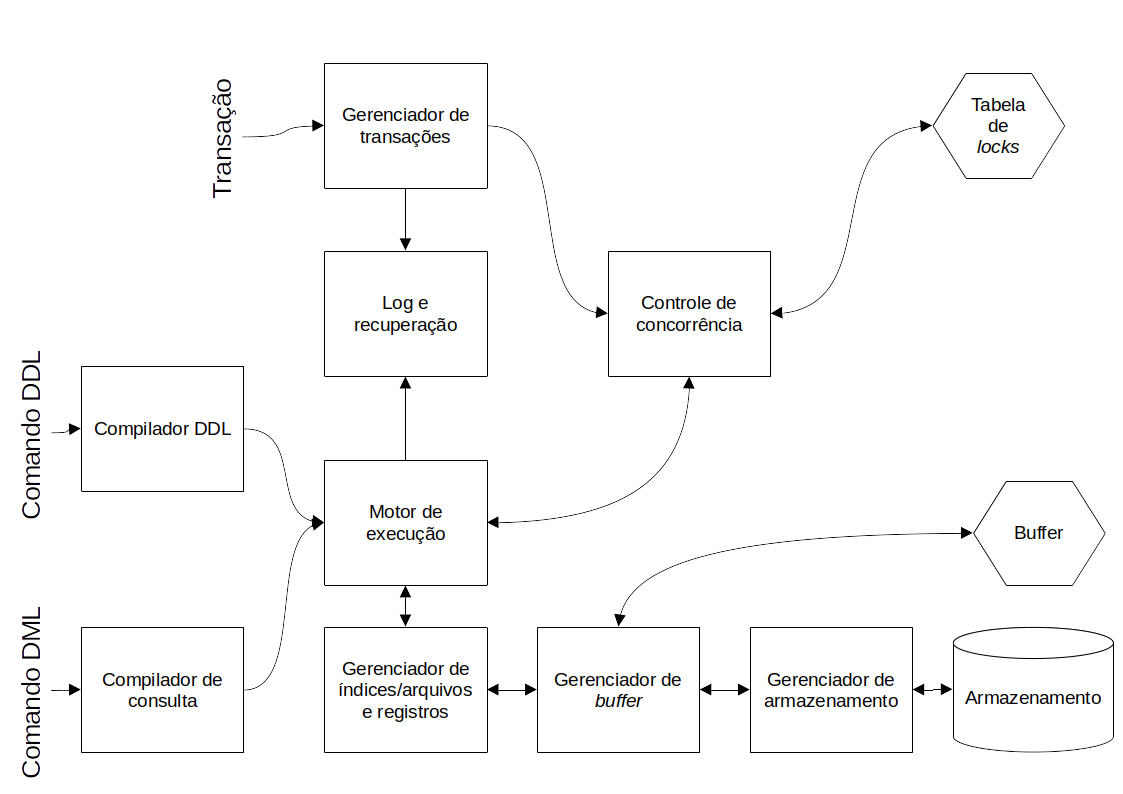
\includegraphics[width=8cm, height=4cm]{figures/database_overview.png}
    \end{figure}\footnote{Adaptado de Garcia-Molina (2009).}
\end{frame}

\begin{frame}{Funcionamento do SGBD}
    O modelo supõe dois tipos de comando:
    \begin{itemize}
        \item comandos de modificação do esquema (comandos DDL);
        \item comandos sobre o estado do banco (comando DML).
    \end{itemize}
    \begin{figure}
        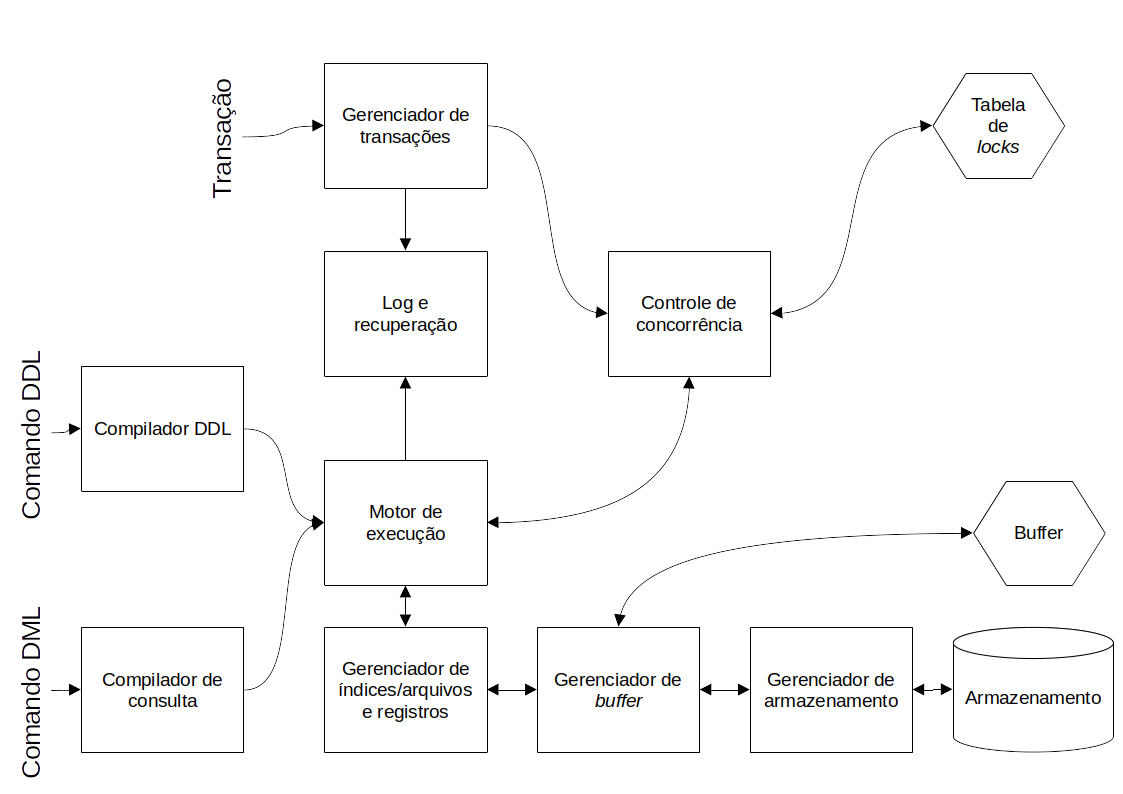
\includegraphics[width=8cm, height=4cm]{figures/database_overview.png}
    \end{figure}
\end{frame}

\begin{frame}{Funcionamento do SGBD}
    \begin{itemize}
        \item O fluxo de execução é bastante similar .
        \item A diferença inicial é que os comando DDL poassam por um compilador DDL e os comandos DML por um compilador de consultas.
        \item Além disso, como os comandos DML modificam o estado da base de dados e comumente são executados em sequência com outros comandos DML, são agrupados em transações.
    \end{itemize}
\end{frame}

\begin{frame}{Funcionamento do SGBD}
    \begin{itemize}
        \item Uma transação é uma sequênciade comandos DML válidos com objetivo específico.
        \item É desejável que um SGBD garanta que as transações tenham propriedades ACID.
    \end{itemize}
\end{frame}

\begin{frame}{Funcionamento do SGBD}
    \begin{itemize}
        \item O comando DML (consulta) é otimizado pelo compilador de consulta com base na \textit{metadata} e em estatísticas.
        \item O resultado da compilação é uma sequência de ações que devem ser realizadas pelo SGBD para executar a consulta.
    \end{itemize}
\end{frame}

\begin{frame}{Funcionamento do SGBD}
    \begin{itemize}
        \item O motor de execução requisita ao gerenciador de recursos (índices, arquivos e registros) os dados, registros ou tuplas de uma relação.
        \item As requisições por dados são passadas para o gerenciador de \textit{buffer}, que verifica se os dados estão na memória.
        \item Caso negativo, o gerenciador de \textit{buffer} trás os blocos de dados necessários do disco par a memória através do gerenciador de armazenamento.
    \end{itemize}
\end{frame}

\begin{frame}{Funcionamento do SGBD}
    Para o processamento das transações são executados os seguintes passos:
    \begin{itemize}
        \item \textit{logging}: para garantir as propriedades ACID, o SGBD armazena cada operação sobre o banco em um arquivo de \textit{log}. Em caso de falha, o SGBD pode desfazer operações, garantindo que nenhuma transação será executada em parcialmente ou que o sistema não fique inconsistente;
        \item controle de concorrência: as transações devem ser isoladas. Por isso, usam-se \textit{locks} (armazenados em um tabela na memória principal) para garantir que uma transação não sobrescreva um dado enquanto outras tentam lê-lo;
        \item resolução de impasses: o uso de \textit{locks} pode gerar impasses. Deste modo, o gerenciador de transações pode abortar transações para que outras possam ser executadas.
    \end{itemize}
\end{frame}

\begin{frame}{Referências}
    \begin{itemize}
        \item Elmasri, Ramez e Navathe, Shamkant. Sistemas de banco de dados. 2011. 6ª ed. Pearson.
        \item Garcia-Molina, Hector; Ullman, Jeffrey D.; e Widom, Jennifer. Database Systems: The Complete Book. 2009. 2ed. Pearson.
    \end{itemize}
\end{frame}

\end{document}